\section{Sensado remoto, plataformas (¿?) (Bloque 1)}

\section{Procesamiento de imágenes (Bloque 2)}

\subsection{Filtrado homomórfico (CRICTE 2017)}
\subsection{Procesamiento morfológico (Pasantía)}
\subsection{Invariante de color (paper RSASE)}
\subsection{Machine learning (¿?)}




Las Tesis  en el marco de la Carrera del Doctorado en Ciencias Aplicadas (DCA) deberán ser escritas en idioma Español, utilizando letra tipo Arial, tamaño 11 puntos, y formato de hojas tipo A4, numeradas en el margen inferior derecho, con interlineado 1,5; sin separación automática de sílabas al fin de línea y con los cuatro márgenes de 2,5 cm.

El contenido de las Tesis deberá incluir los siguientes ítems y en el siguiente orden:\newline
●	Carátula (con el formato solicitado por el DCA que se adjunta al presente Anexo)\newline
●	Agradecimientos\newline
●	Índice\newline
●	Listado de Abreviaturas (en caso de que lo considere conveniente)\newline
●	Resumen en Español\newline
●	Palabras Claves en Español (tres a seis palabras claves separadas por comas. La primera letra de cada palabra clave debe empezar con mayúscula)\newline
●	Resumen en Inglés (Abstract)\newline
●	Palabras Claves en Inglés (tres a seis palabras claves separadas por comas. La primera letra de cada palabra clave debe empezar con mayúscula)\newline
●	Capítulo 1: Introducción (deberá contener el planteo del problema a resolver, los objetivos generales y específicos y una breve explicación de lo que versará la Tesis)\newline
●	Capítulo 2: Marco Teórico\newline
●	Capítulo 3: Metodología\newline
●	Capítulo 4: Resultados y Discusión (O bien, se podrá presentar en dos Capítulos separados: Capítulo 4: Resultados y Capítulo 5: Discusión)\newline
●	Capítulo 5: Conclusiones (Deben presentarse en párrafos cortos y concretos. No deben hacer referencia a trabajos futuros ni a hipótesis no incluidas en el trabajo).\newline
●	Recomendaciones para Trabajos Futuros\newline
●	Producción Científica (surgida del trabajo de Tesis)\newline
✔	Publicaciones en Revistas y Capítulos de Libros\newline
✔	Presentaciones a Congresos\newline
●	Proyecto/s de Investigación dentro del/los cual/es se desarrolló la Tesis (si hubiera/n)\newline
●	Beca/s y Subsidio/s con los que se financió la Tesis (si hubieran)\newline
●	Apéndices o Anexos (se reservan para detallar técnicas originales utilizadas o análisis teóricos que impedirían seguir fluidamente el trabajo si se incluyeran en el texto). Las tablas y figuras de los apéndices o anexos deben comenzar otra numeración diferente a la de los capítulos.\newline

Aclaraciones

⮚	El listado de Referencias bibliográficas se podrá incorporar al final de cada capítulo, ó todas juntas al final de la Tesis, las mismas serán listadas en el orden en que aparecen citadas en el texto. \newline
Formato de las Referencias\newline
Estilo de las Referencias\newline
En el texto de la Tesis: indique las referencias por número (s) entre corchetes en línea con el texto. Cuando se menciona a los autores, siempre se deben proporcionar los números de referencia.
Ejemplo: '..... como se demostró [3,6]. Barnaby y Jones [8] obtuvieron un resultado diferente ... '
Lista de Referencias\newline
Numere las referencias (números entre corchetes) en la lista en el orden en que aparecen en el texto, como se indica a continuación:
\paragraph{Referencia a una publicación de revista}
[1] J. van der Geer, J.A.J. Hanraads, R.A. Lupton, The art of writing a scientific article, J. Sci. Commun. 163 (2010) 51–59.https://doi.org/10.1016/j.Sc.2010.00372.
\paragraph{Referencia a una publicación de revista con un número de artículo}
[2] J. van der Geer, J.A.J. Hanraads, R.A. Lupton, 2018. The art of writing a scientific article.Heliyon. 19, e00205.https://doi.org/10.1016/j.heliyon.2018.e00205.
\paragraph{Referencia a un libro}
[3] W. Strunk Jr., E.B. White, The Elements of Style, fourth ed., Longman, New York, 2000.
\paragraph{Referencia a un capítulo en un libro editado}
[4] G.R. Mettam, L.B. Adams, How to prepare an electronic version of your article, in: B.S. Jones, R.Z. Smith (Eds.), Introduction to the Electronic Age, E-Publishing Inc., New York, 2009, pp. 281–304.
\paragraph{Referencia a un sitio} web
[5] Cancer Research UK, Cancer statistics reports for the UK. http://www.cancerresearchuk.org/ aboutcancer/statistics/cancerstatsreport/, 2003 (accessed 13 March 2003).
\paragraph{Referencia a un conjunto de datos: [conjunto de datos]}
[6] M. Oguro, S. Imahiro, S. Saito, T. Nakashizuka, Mortality data for Japanese oak wilt disease and surrounding forest compositions, Mendeley Data, v1, 2015. https://doi.org/10.17632/ xwj98nb39r.1
⮚	Las figuras (gráficos, cuadros, fotografías, otros) deberán numerarse correlativamente en el orden de aparición en el texto y deberán incluir un breve título explicativo en la parte inferior de la figura. Las imágenes y fotografías se designarán como figuras.\newline
%%%%%%%%%%%%%%%%%%%%%%%%%%%%%%%%%%%%%%% FIGURA %%%%%%%%%%%%%%%%%%%%%%%%%%%%%%%%%%%%%%%%%%%%%%%%%%%%%%%%%
%\begin{figure}[ht!]
%    \centering
%    \captionsetup{justification=centering}
%    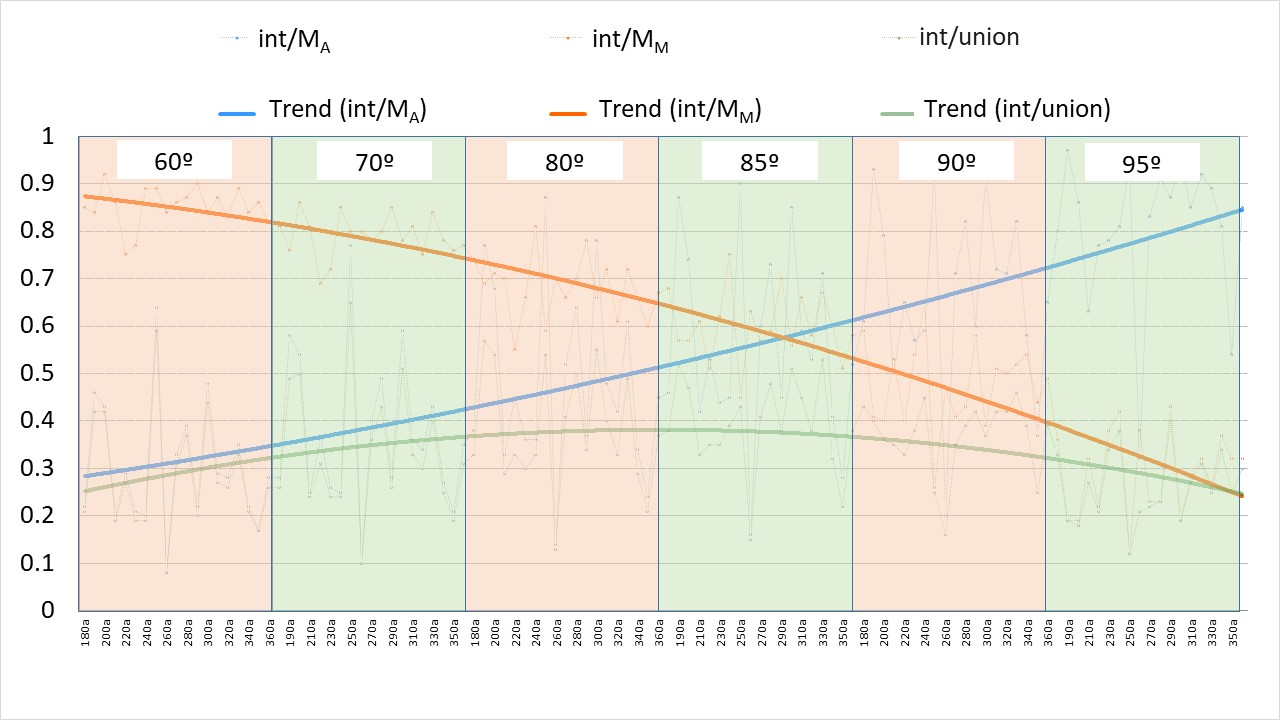
\includegraphics[width=8cm]{grafico.jpg}
%    \caption{Quality Index as a function of the percentile, for the different forest image used. QI\textsubscript{1} in orange, QI\textsubscript{2} in blue and QI\textsubscript{3} in green. The invariant color index used is ψ\textsubscript{BR}}	
 %   \label{qi}
%\end{figure}
%%%%%%%%%%%%%%%%%%%%%%%%%%%%%%%%%%%%%%%%%%%%%%%%%%%%%%%%%%%%%%%%%%%%%%%%%%%%%%%%%%%%%%%%%%%%%%%%%%%%%%%%%
⮚	Las tablas deberán numerarse correlativamente según su orden de aparición en el texto y en forma independiente de las figuras. Deberán incluir un título explicativo en su parte superior. De ser necesario se agregarán al pie notas explicativas para detallar abreviaturas, signos, medidas, otros, de tal manera que el lector pueda comprender su contenido sin recurrir al texto.
%%%%%%%%%%%%%%%%%%%%%%%%%%%%%%%%%%%%%%%%% TABLA %%%%%%%%%%%%%%%%%%%%%%%%%%%%%%%%%%%%%%%%%%%%%%%%%%%%%%%%%
\begin{table}[H]
    \centering
    \caption{Evaluation of the superposition of both masks. the manual and the automatic. carried on by the group of experts}
    \begin{tabular}{|c|c|c|c|c|c|c|c|}
       \hline
        COLOR INVARIANT INDEX & \multicolumn{6}{ |c|}{\textpsi \textsubscript{BR}}\\%\multicolumn{6}{ }{ |c|} \\
        \hline
        PERCENTILE & 60 & 70 & 80 & 85 & 90 & 95\\
        \hline
        GOOD & 0.0 & 0.0 & 4.5 & 15.8 & 20.5 & 0.0\\
        \hline
        REGULAR & 0.0 & 4.5 & 27.3 & 21.1 & 54.5 & 57.9\\
        \hline
        BAD & 100.0 & 95.5 & 68.2 & 63.2 & 25.0 & 42.1\\
        \hline
        COLOR INVARIANT INDEX & \multicolumn{6}{ |c|}{\textpsi \textsubscript{BG}}\\
        \hline
        PERCENTILE & 60 & 70 & 80 & 85 & 90 & 95\\
        \hline
        GOOD & 0.0 & 0.0 & 0.0 & 5.3 & 5.3 & 5.3\\
        \hline
        REGULAR & 0.0 & 5.3 & 10.5 & 15.8 & 42.1 & 21.1\\
        \hline
        BAD & 100.0 & 94.7 & 89.5 & 78.9 & 52.6 & 73.7\\
        \hline
        COLOR INVARIANT INDEX & \multicolumn{6}{|c|}{ \textpsi \textsubscript{GR}}\\
        \hline
        PERCENTILE & 60 & 70 & 80 & 85 & 90 & 95\\
        \hline
        GOOD & 0.0 & 0.0 & 0.0 & 0.0 & 0.0 & 0.0\\
        \hline
        REGULAR & 0.0 & 0.0 & 0.0 & 0.0 & 15.8 & 15.8\\
        \hline
        BAD & 100.0 & 100.0 & 100.0 & 100.0 & 84.2 & 84.2\\
        \hline
    \end{tabular}
    \\
    \raggedleft
    \label{tablita}
\end{table}
%%%%%%%%%%%%%%%%%%%%%%%%%%%%%%%%%%%%%%%%%%%%%%%%%%%%%%%%%%%%%%%%%%%%%%%%%%%%%%%%%%%%%%%%%%%%%%%%%%%%%%%%%
⮚	Las fórmulas y expresiones matemáticas deberán ser escritas dejando dos espacios sobre, debajo y entre cada una de ellas.
%%%%%%%%%%%%%%%%%%%%%%%%%%%%%%%%%%%%%% ECUACIÓN %%%%%%%%%%%%%%%%%%%%%%%%%%%%%%%%%%%%%%%%%%%%%%%%%%%%%%%%%
\begin{equation}
	\psi=\frac{4}{\pi} arctan\left(\frac{B\textsubscript{1}-B\textsubscript{2}}{B\textsubscript{1}+B\textsubscript{2}}\right),\label{eq1}
\end{equation}
%%%%%%%%%%%%%%%%%%%%%%%%%%%%%%%%%%%%%%%%%%%%%%%%%%%%%%%%%%%%%%%%%%%%%%%%%%%%%%%%%%%%%%%%%%%%%%%%%%%%%%%%%
Las fórmulas se ajustarán al margen izquierdo y serán numeradas correlativamente y entre paréntesis sobre el margen derecho. Debe quedar definido el significado y las unidades utilizadas en cada término de las expresiones.

⮚	Unidades: debe utilizarse el sistema internacional de unidades (SI).
